\documentclass[specification,annotation,times]{itmo-student-thesis}

%% Опции пакета:
%% - specification - если есть, генерируется задание, иначе не генерируется
%% - annotation - если есть, генерируется аннотация, иначе не генерируется
%% - times - делает все шрифтом Times New Roman, собирается с помощью xelatex
%% - pscyr - делает все шрифтом Times New Roman, требует пакета pscyr.

%% Делает запятую в формулах более интеллектуальной, например:
%% $1,5x$ будет читаться как полтора икса, а не один запятая пять иксов.
%% Однако если написать $1, 5x$, то все будет как прежде.
\usepackage{icomma}

%% Данные пакеты необязательны к использованию в бакалаврских/магистерских
%% Они нужны для иллюстративных целей
%% Начало
\usepackage{tikz}
\usetikzlibrary{arrows}
%% Конец

%% Указываем файл с библиографией.
\addbibresource{master-thesis.bib}

\begin{document}

\studygroup{M4239}
\title{Децентрализованный алгоритм управления конвейерной системой с использованием методов мультиагентного обучения с подкреплением}
\author{Мухутдинов Дмитрий Вадимович}{Мухутдинов Д.В.}
\supervisor{Фильченков Андрей Александрович}{Фильченков А.А.}{канд. физ.-мат. наук}{кафедра КТ}
\publishyear{2019}
%% Дата выдачи задания. Можно не указывать, тогда надо будет заполнить от руки.
\startdate{01}{сентября}{2017}
%% Срок сдачи студентом работы. Можно не указывать, тогда надо будет заполнить от руки.
\finishdate{31}{мая}{2019}
%% Дата защиты. Можно не указывать, тогда надо будет заполнить от руки.
\defencedate{15}{июня}{2019}

\addconsultant{Вяткин В.В.}{докт. техн. наук, проф.}

\secretary{Павлова О.Н.}

%% Задание
%%% Техническое задание и исходные данные к работе
\technicalspec{Требуется разработать децентрализованный алгоритм управления
  конвейерной системы для транспортировки багажа. Алгоритм должен позволять
  контроллерам конвейерной сети динамически изменять свое поведение в целях
  адаптации под изменившиеся условия работы, такие как поломка одного из
  конвейеров или изменение интенсивности потока багажа. Алгоритм должен
  обеспечивать своевременную доставку багажных единиц до пунктов назначения, в
  то же время минимизируя энергопотребление всей системы в целом.
}

%%% Содержание выпускной квалификационной работы (перечень подлежащих разработке вопросов)
\plannedcontents{Пояснительная записка должна содержать обзор существующих
  результатов в сфере управления конвейерными системами, а также в сферах,
  имеющих непосредственное отношение к предложенному алгоритму (таких как
  обучение с подкреплением). Также записка должна содержать подробное изложение
  предложенного алгоритма и данные экспериментального сравнения его
  производительности с производительностью существующих методов управления
  конвейерной системой, проведенного с помощью виртуальной имитационной модели
  конвейерной сети.
}

%%% Исходные материалы и пособия 
\plannedsources{\begin{enumerate}
  \item Richard S. Sutton and Andrew G. Barto. Reinforcement Learning: An Introduction. The MIT Press, 2012
  \item Mnih et al. Human-level control through deep reinforcement learning. Nature, 518(7540):529–533, 2015.
\end{enumerate}}

%%% Календарный план
\addstage{Ознакомление с предметной областью}{11.2017}
\addstage{Чтение статей, посвященных алгоритмам маршрутизации}{01.2018}
\addstage{Чтение статей, посвященных задаче обучения с подкреплением}{02.2018}
\addstage{Чтение статей, посвященных задаче обучения с подкреплением}{03.2018}
\addstage{Чтение статей, посвященных задаче управления конвейерными системами}{05.2018}
\addstage{Разработка имитационной модели конвейерной сети}{09.2018}
\addstage{Реализация существующих алгоритмов управления}{11.2018}
\addstage{Разработка алгоритма маршрутизации, проведение экспериментов}{03.2019}
\addstage{Написание пояснительной записки}{05.2019}

%%% Цель исследования
\researchaim{Разработка удобного стилевого файла \LaTeX
             для бакалавров и магистров кафедры компьютерных технологий.}

%%% Задачи, решаемые в ВКР
\researchtargets{\begin{enumerate}
    \item соответствие титульной страницы, задания и аннотации шаблонам, принятым в настоящее время на
    кафедре;
    \item соответствие содержательной части пояснительной записки требованиям ГОСТ~7.0.11-2011 <<Диссертация и
    автореферат диссертации>>;
    \item относительное удобство в использовании~--- указание данных об авторе и научном руководителе один раз
    и в одном месте, автоматический подсчет числа тех или иных источников.
\end{enumerate}}

%%% Использование современных пакетов компьютерных программ и технологий
\advancedtechnologyusage{
  Программный код имитационной модели конвейерной сети и алгоритмов управления
  написан на языке Python 3.6. При разработке имитационной модели конвейерной
  системы была использована библиотека для дискретно-событийного моделирования
  SimPy. Программный код алгоритмов управления конвейерной системой использует
  библиотеки NetworkX, NumPy, SciPy, scikit-learn, PyTorch. Для проведения
  экспериментальных исследований использовалась система интерактивной разработки
  Jupyter Lab и библиотеки matplotlib, pandas, tqdm.
}

%%% Краткая характеристика полученных результатов 
\researchsummary{
  Разработан алгоритм управления конвейерной системой на основе глубокого
  мультиагентного обучения с подкреплением. В ходе экспериментального
  исследования было установлено, что разработанный алгоритм превосходит
  существующие по качеству работы и способен адаптироваться к изменениям во
  внешней среде.
}

%%% Гранты, полученные при выполнении работы 
\researchfunding{
  TBD: вписать грант?
}

%%% Наличие публикаций и выступлений на конференциях по теме выпускной работы
\researchpublications{
\begin{refsection}
\nocite{mukhutdinov2019multi}
\printannobibliography
\end{refsection}
}

%% Эта команда генерирует титульный лист и аннотацию.
\maketitle{Магистр}

%% Оглавление
\tableofcontents

%% Макрос для введения. Совместим со старым стилевиком.
\startprefacepage

В данном разделе размещается введение.

%% Начало содержательной части.
\chapter{Первая глава}

%% Так помечается начало обзора.
\startrelatedwork
Пример ссылок в рамках обзора: \cite{vyatkin-controllers, q-routing-orig, tan1993multi}.
%% Так помечается конец обзора.
\finishrelatedwork
Вне обзора:~\cite{bellman}.

\section{Таблицы}

В качестве примера таблицы приведена таблица~\ref{tab1}.

\begin{table}[!h]
\caption{Таблица умножения (фрагмент)}\label{tab1}
\centering
\begin{tabular}{|*{18}{c|}}\hline
-- & 1 & 2 & 3 & 4 & 5 & 6 & 7 & 8 & 9 & 10 & 11 & 12 & 13 & 14 & 15 & 16 & 17 \\\hline
1  & 1 & 2 & 3 & 4 & 5 & 6 & 7 & 8 & 9 & 10 & 11 & 12 & 13 & 14 & 15 & 16 & 17 \\\hline
2  & 2 & 4 & 6 & 8 & 10 & 12 & 14 & 16 & 18 & 20 & 22 & 24 & 26 & 28 & 30 & 32 & 34 \\\hline
3  & 3 & 6 & 9 & 12 & 15 & 18 & 21 & 24 & 27 & 30 & 33 & 36 & 39 & 42 & 45 & 48 & 51 \\\hline
4  & 4 & 8 & 12 & 16 & 20 & 24 & 28 & 32 & 36 & 40 & 44 & 48 & 52 & 56 & 60 & 64 & 68 \\\hline
\end{tabular}
\end{table}

Есть еще такое окружение \texttt{tabu}, его можно аккуратно растянуть на всю страницу.
Приведем пример (таблица~\ref{tab2}).

\begin{table}[!h]
\caption{Таблица умножения с помощью \texttt{tabu} (фрагмент)}\label{tab2}
\centering
\begin{tabu}{|*{18}{X[c]|}}\hline
-- & 1 & 2 & 3 & 4 & 5 & 6 & 7 & 8 & 9 & 10 & 11 & 12 & 13 & 14 & 15 & 16 & 17 \\\hline
1  & 1 & 2 & 3 & 4 & 5 & 6 & 7 & 8 & 9 & 10 & 11 & 12 & 13 & 14 & 15 & 16 & 17 \\\hline
2  & 2 & 4 & 6 & 8 & 10 & 12 & 14 & 16 & 18 & 20 & 22 & 24 & 26 & 28 & 30 & 32 & 34 \\\hline
3  & 3 & 6 & 9 & 12 & 15 & 18 & 21 & 24 & 27 & 30 & 33 & 36 & 39 & 42 & 45 & 48 & 51 \\\hline
4  & 4 & 8 & 12 & 16 & 20 & 24 & 28 & 32 & 36 & 40 & 44 & 48 & 52 & 56 & 60 & 64 & 68 \\\hline
\end{tabu}
\end{table}

\section{Рисунки}

Пример рисунка (c помощью \texttt{TikZ}) приведен на рисунке~\ref{fig1}. Под \texttt{pdflatex} можно также
использовать \texttt{*.jpg}, \texttt{*.png} и даже \texttt{*.pdf}, под \texttt{latex} можно использовать
Metapost. Последний можно использовать и под \texttt{pdflatex}, для чего в стилевике продекларированы
номера картинок от~1 до~20.

\begin{figure}[!h]
\caption{Пример рисунка}\label{fig1}
\centering
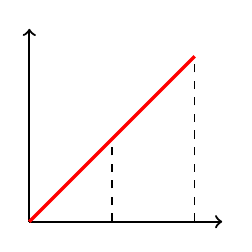
\begin{tikzpicture}[scale=0.7]
\draw[thick,->] (0,0)--(3.5,0);
\draw[thick,->] (0,0)--(0,3.5);
\draw[very thick, red] (0,0)--(3,3);
\draw[dashed] (3,0)--(3,3);
\draw[dashed] (1.5,0)--(1.5,1.5);
\end{tikzpicture}
\end{figure}

\section{Листинги}

В работах студентов кафедры <<Компьютерные технологии>> часто встречаются листинги. Листинги бывают
двух основных видов~--- исходный код и псевдокод. Первый оформляется с помощью окружения \texttt{lstlisting}
из пакета \texttt{listings}, который уже включается в стилевике и немного настроен. Пример Hello World на Java
приведен на листинге~\ref{lst1}. Пример большого листинга~--- в приложении (листинг~\ref{lstX}).

\begin{lstlisting}[float=!h,caption={Пример исходного кода на Java},label={lst1}]
public class HelloWorld {
	public static void main(String[] args) {
		System.out.println("Hello, world!");
	}
}
\end{lstlisting}

Псевдокод можно оформлять с помощью разных пакетов. В данном стилевике включается пакет \texttt{algorithmicx}.
Сам по себе он не генерирует флоатов, поэтому для них используется пакет \texttt{algorithm}.
Пример их совместного использования приведен на листинге~\ref{lst2}.

\begin{algorithm}[!h]
\caption{Пример псевдокода}\label{lst2}
\begin{algorithmic}
	\Function{IsPrime}{$N$}
		\For{$t \gets [2; \lfloor\sqrt{N}\rfloor]$}
			\If{$N \bmod t = 0$}
				\State\Return \textsc{false}
			\EndIf
		\EndFor
		\State\Return \textsc{true}
	\EndFunction
\end{algorithmic}
\end{algorithm}

Наконец, листинги из \texttt{listings} тоже можно подвешивать с помощью \texttt{algorithm},
пример на листинге~\ref{lst3}.

\begin{algorithm}[!h]
\caption{Исходный код и флоат \texttt{algorithm}}\label{lst3}
\begin{lstlisting}
public class HelloWorld {
	public static void main(String[] args) {
		System.out.println("Hello, world!");
	}
}
\end{lstlisting}
\end{algorithm}

\chapter{Проверка сквозной нумерации}

Листинг~\ref{lst4} должен иметь номер 4.

\begin{algorithm}[!h]
\caption{Исходный код и флоат \texttt{algorithm}}\label{lst4}
\begin{lstlisting}
public class HelloWorld {
	public static void main(String[] args) {
		System.out.println("Hello, world!");
	}
}
\end{lstlisting}
\end{algorithm}

Рисунок~\ref{fig2} должен иметь номер 2.

\begin{figure}[!h]
\caption{Пример рисунка}\label{fig2}
\centering
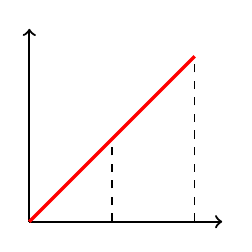
\begin{tikzpicture}[scale=0.7]
\draw[thick,->] (0,0)--(3.5,0);
\draw[thick,->] (0,0)--(0,3.5);
\draw[very thick, red] (0,0)--(3,3);
\draw[dashed] (3,0)--(3,3);
\draw[dashed] (1.5,0)--(1.5,1.5);
\end{tikzpicture}
\end{figure}

Таблица~\ref{tab3} должна иметь номер 3.

\begin{table}[!h]
\caption{Таблица умножения с помощью \texttt{tabu} (фрагмент)}\label{tab3}
\centering
\begin{tabu}{|*{18}{X[c]|}}\hline
-- & 1 & 2 & 3 & 4 & 5 & 6 & 7 & 8 & 9 & 10 & 11 & 12 & 13 & 14 & 15 & 16 & 17 \\\hline
1  & 1 & 2 & 3 & 4 & 5 & 6 & 7 & 8 & 9 & 10 & 11 & 12 & 13 & 14 & 15 & 16 & 17 \\\hline
2  & 2 & 4 & 6 & 8 & 10 & 12 & 14 & 16 & 18 & 20 & 22 & 24 & 26 & 28 & 30 & 32 & 34 \\\hline
3  & 3 & 6 & 9 & 12 & 15 & 18 & 21 & 24 & 27 & 30 & 33 & 36 & 39 & 42 & 45 & 48 & 51 \\\hline
4  & 4 & 8 & 12 & 16 & 20 & 24 & 28 & 32 & 36 & 40 & 44 & 48 & 52 & 56 & 60 & 64 & 68 \\\hline
\end{tabu}
\end{table}

\chapterconclusion

В конце каждой главы желательно делать выводы. Вывод по данной главе~--- нумерация работает корректно, ура!

%% Макрос для заключения. Совместим со старым стилевиком.
\startconclusionpage

В данном разделе размещается заключение.

%% Обратите внимание на heading. Без него тоже работает, но название будет другим.
\printmainbibliography

%% После этой команды chapter будет генерировать приложения, нумерованные русскими буквами.
%% \startappendices из старого стилевика будет делать то же самое
\appendix

\chapter{Пример приложения}

В приложениях рисунки, таблицы и другие подобные элементы нумеруются по приложениям с соответствующим префиксом. Проверим это.

Листинг~\ref{lst4:apx} должен иметь номер А.1.

\begin{algorithm}[!h]
\caption{Исходный код и флоат \texttt{algorithm}}\label{lst4:apx}
\begin{lstlisting}
public class HelloWorld {
    public static void main(String[] args) {
        System.out.println("Hello, world!");
    }
}
\end{lstlisting}
\end{algorithm}

Рисунок~\ref{fig2:apx} должен иметь номер A.1.

\begin{figure}[!h]
\caption{Пример рисунка}\label{fig2:apx}
\centering
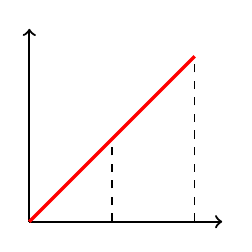
\begin{tikzpicture}[scale=0.7]
\draw[thick,->] (0,0)--(3.5,0);
\draw[thick,->] (0,0)--(0,3.5);
\draw[very thick, red] (0,0)--(3,3);
\draw[dashed] (3,0)--(3,3);
\draw[dashed] (1.5,0)--(1.5,1.5);
\end{tikzpicture}
\end{figure}

Таблица~\ref{tab3:apx} должна иметь номер A.1.

\begin{table}[!h]
\caption{Таблица умножения с помощью \texttt{tabu} (фрагмент)}\label{tab3:apx}
\centering
\begin{tabu}{|*{18}{X[c]|}}\hline
-- & 1 & 2 & 3 & 4 & 5 & 6 & 7 & 8 & 9 & 10 & 11 & 12 & 13 & 14 & 15 & 16 & 17 \\\hline
1  & 1 & 2 & 3 & 4 & 5 & 6 & 7 & 8 & 9 & 10 & 11 & 12 & 13 & 14 & 15 & 16 & 17 \\\hline
2  & 2 & 4 & 6 & 8 & 10 & 12 & 14 & 16 & 18 & 20 & 22 & 24 & 26 & 28 & 30 & 32 & 34 \\\hline
3  & 3 & 6 & 9 & 12 & 15 & 18 & 21 & 24 & 27 & 30 & 33 & 36 & 39 & 42 & 45 & 48 & 51 \\\hline
4  & 4 & 8 & 12 & 16 & 20 & 24 & 28 & 32 & 36 & 40 & 44 & 48 & 52 & 56 & 60 & 64 & 68 \\\hline
\end{tabu}
\end{table}

Заодно проверим нумерованные и ненумерованные перечисления. Ненумерованные:
\begin{itemize}
    \item пункт А;
    \item пункт Б;
    \item пункт В.
\end{itemize}

Нумерованные списки нескольких уровней:
\begin{enumerate}
    \item первый элемент;
    \item второй элемент с подэлементами:
    \begin{enumerate}
        \item первый подэлемент;
        \item второй подэлемент;
        \item третий подэлемент.
    \end{enumerate}
    \item третий элемент;
    \item четвертый элемент;
    \item пятый элемент;
    \item шестой элемент;
    \item седьмой элемент;
    \item восьмой элемент;
    \item девятый элемент;
    \item десятый элемент.
\end{enumerate}

\chapter{Еще один пример приложения с неимоверно длиннющим названием для тестирования переносов}

Проверим на примере таблиц, что нумерация в приложениях~--- по приложениям.
Таблица~\ref{tab3:apx2} должна иметь номер Б.1.

\begin{table}[!h]
\caption{Таблица умножения с помощью \texttt{tabu} (фрагмент)}\label{tab3:apx2}
\centering
\begin{tabu}{|*{18}{X[c]|}}\hline
-- & 1 & 2 & 3 & 4 & 5 & 6 & 7 & 8 & 9 & 10 & 11 & 12 & 13 & 14 & 15 & 16 & 17 \\\hline
1  & 1 & 2 & 3 & 4 & 5 & 6 & 7 & 8 & 9 & 10 & 11 & 12 & 13 & 14 & 15 & 16 & 17 \\\hline
2  & 2 & 4 & 6 & 8 & 10 & 12 & 14 & 16 & 18 & 20 & 22 & 24 & 26 & 28 & 30 & 32 & 34 \\\hline
3  & 3 & 6 & 9 & 12 & 15 & 18 & 21 & 24 & 27 & 30 & 33 & 36 & 39 & 42 & 45 & 48 & 51 \\\hline
4  & 4 & 8 & 12 & 16 & 20 & 24 & 28 & 32 & 36 & 40 & 44 & 48 & 52 & 56 & 60 & 64 & 68 \\\hline
\end{tabu}
\end{table}

\chapter{Пример огромного листинга}

\begin{lstlisting}[caption={Пример большого листинга},label={lstX}]
import java.util.*;

public class Example {
    static int[] restoreOutgoing(int[] g, int[] outgoing,
                                 int vertex, int mask) {
        int[] rv = new int[1 + Integer.bitCount(mask)];
        int n = g.length;
        int current = rv.length - 1;
        while (true) {
            rv[current] = vertex;
            if (current == 0) {
                if (vertex != 0) {
                    throw new AssertionError();
                }
                return rv;
            }
            mask ^= 1 << (vertex - 1);
            int prevMask = outgoing[mask] & g[vertex];
            if (prevMask == 0) {
                throw new AssertionError();
            }
            vertex = Integer.numberOfTrailingZeros(prevMask);
            --current;
        }
    }

    static int[] restoreIncoming(int[] g, int[] incoming,
                                 int vertex, int mask) {
        int[] rv = new int[1 + Integer.bitCount(mask)];
        int n = g.length;
        int current = 0;
        while (true) {
            rv[current] = vertex;
            if (current == rv.length - 1) {
                if (vertex != 0) {
                    throw new AssertionError();
                }
                return rv;
            }
            mask ^= 1 << (vertex - 1);
            int nextMask = incoming[mask] & g[vertex];
            if (nextMask == 0) {
                throw new AssertionError();
            }
            vertex = Integer.numberOfTrailingZeros(nextMask);
            ++current;
        }
    }
}
\end{lstlisting}
                

\end{document}
